\documentclass{ddis-thesis}
\usepackage{amsmath, amsthm, amssymb}
\usepackage[latin1]{inputenc}
\usepackage{program}
\usepackage{mathrsfs}
\usepackage{amsfonts}
\usepackage{algorithm}
\usepackage[noend]{algpseudocode}
\usepackage{graphicx}

\usepackage{fancyvrb}
\DefineVerbatimEnvironment{code}{Verbatim}{fontsize=\small}
\DefineVerbatimEnvironment{example}{Verbatim}{fontsize=\small}

\makeatletter
\def\BState{\State\hskip-\ALG@thistlm}
\makeatother

\usepackage{fancyhdr}% fancyhdr related command; details in its documentation
\pagestyle{fancy}
\fancyhead{}
\fancyhead[LE,RO]{\thepage}
\fancyhead[RE]{\leftmark}
\fancyhead[LO]{\rightmark}


\usepackage{graphicx}
\author{name}
\title{Dynamic Constraint Optimization}
\begin{document}

% *************** Front matter ***************

\frontmatter
\begin{titlepage}

\setlength{\textwidth}{16cm}
\setlength{\oddsidemargin}{0cm}
\setlength{\evensidemargin}{0cm}
\setlength{\topmargin}{8mm}
\setlength{\headheight}{0cm}
\setlength{\headsep}{0cm}
\setlength{\topskip}{0cm}
\enlargethispage{5cm}

\noindent
\setlength{\unitlength}{1mm}

\begin{picture}(160,226)
\centering

\put(0,203){\line(1,0){160}} % lower line
\put(109,39){\line(1,0){50}}
\put(109,161){\line(1,0){50}}
\put(109,170){\line(1,0){50}}
\put(107,1){\line(0,1){200}}

\put(0,140){\parbox[b]{100mm}{
    \begin{center}
    {\bf\Huge {\sffamily{Dynamic Distributed Constraint Optimization}}}
    \end{center}}}


\put(109,92){\parbox[b]{50mm}{
    {\bf
    {\sffamily{{\Large Daniel Hegglin}}}}\\
    {\sffamily{of Oerlikon ZH, Switzerland\\\\
    Student-ID: 08-721-102\\
    dani.hegglin@gmail.com
    }}
}}

\put(109,161){\makebox(50,9){{\sffamily{Thesis \hfill\today}}}}

\put(0,215){\makebox(80,11)[l]{
\includegraphics[height=2.8cm]
{./section-title/figures/uzh_logo_e_pos}}}


\put(109,32){\parbox[b]{50mm}{\flushleft
    {\sffamily{Advisor:}} {\bf {\sffamily{Mihaela Verman}} }
    }
}

\put(109,10){\parbox[b]{50mm}{\flushleft
        {\sffamily{
        Prof. Abraham Bernstein, PhD\\
        Institut f\"ur Informatik\\
        Universit\"at Z\"urich\\
        http://www.ifi.uzh.ch/ddis}
        }
}}

\end{picture}
\end{titlepage}



\begin{acknowledgements}
Lorem ipsum dolor sit amet, consectetuer adipiscing elit. Nullam a tellus.
Aliquam commodo dui non ipsum. Duis mollis nisi id turpis. Donec quis ipsum.
Curabitur sed nibh. Morbi suscipit justo quis orci. Ut massa tortor, ultricies
vitae, lacinia eu, facilisis eu, nisl. Nulla mattis urna sed metus imperdiet
ornare. Praesent sodales. Etiam laoreet. Mauris quam magna, sagittis et,
pharetra eget, congue vitae, arcu. Fusce sollicitudin justo. Suspendisse
lectus. Sed lobortis dolor quis lectus scelerisque ornare. Integer purus.
Phasellus vel elit at nibh sagittis lobortis. Aliquam iaculis malesuada eros.
Mauris metus
\end{acknowledgements}

\begin{zusammenfassung}
Distributed Constraint Optimization (DCOP) erm{\"o}glicht Probleml{\"o}sungen in beispielweise Terminplanung, Verkehrsflusskontrolle oder dem Management von Sensor Netzwerken. Es ist ein gut erforschtes Feld und es wurden viele verschieden Algorithmen zur Berechnung vorgestellt. Allerdings wird h{\"a}ufig von einer statischen Problemdefinition ausgegangen und der Aspekt von in der Realit{\"a}t h{\"a}ufig auftretenden {\"A}nderungen an der Problemstellung findet oft wenig Beachtung. Ausserdem fehlt es an einem soliden theoretischen Fundament und standardisierten Verfahren um die Performanz von DCOP Algorithmen hinsichtlich sich {\"a}ndernder Probleme zu erfassen. Diese Arbeit hatte das Ziel das Verhalten und die Leistung von verschieden Arten von DCOP Algorithmen in dynamischen Umgebungen mit einem Fokus auf lokale, iterative Algorithmen und Hauptaugenmerk auf den MaxSum Algorithmus zu untersuchen. Zum Vergleich wurde eine komplette und eine lokal, iterative "message-passing" sowie eine "best-response" Variante implementiert. W{\"a}hrend der Implementation des MaxSum Algorithmus wurde eine Variation von der {\"u}blichen Graphenstruktur ausprobiert. Zum Test eines realen Problems wurde Terminplanung ausgew{\"a}hlt und als DCOP formuliert. Es wurde ausserdem ein Framework entwickelt, welches die dynamische {\"A}nderung von Constraints, Variablen und der Problemdom{\"a}ne erm{\"o}glicht. Die Algorithmen wurden mit Fokus auf L{\"o}sungs-Qualit{\"a}t {\"u}ber Zeit, sowohl in einer statischen wie auch in einer dynamischen Umgebung getestet. Diese Arbeit schl{\"a}gt ausserdem eine L{\"o}sung zur Speicherung, Weiterverarbeitung und {\"U}berwachung der Resultate der Berechnungen in Echtzeit vor, welche die Performanz der Algorithmen nicht beeinflusst.
\end{zusammenfassung}



\begin{abstract}
Distributed constraint optimization allows to solve problems in domains like scheduling, traffic flow management or sensor network management. It is a well-researched field and various algorithms have been proposed. However, the dynamic nature of some of these problems in the real world have been overlooked by researchers and problems are often assumed to be static during the course of the computation. The benchmarking of distributed constraint optimization algorithms (DCOP) with changing problem definitions currently lacks a solid theoretical foundation and standardized protocols. This thesis aimed to measure the performance of different types of DCOP algorithms on dynamic problems with a focus on local-iterative algorithms and especially on the MaxSum algorithm and possibly contribute to the field. A complete, a local-iterative message-passing and a local-iterative approximate best-response algorithm for distributed constraint optimization have been implemented for comparison.  In the implementation of the MaxSum algorithm, a variation of the usual graph structure has been attempted.  As a real-world use case for benchmarking, the meeting scheduling problem has been mapped as distributed constraint optimization problem. A framework has been designed that allows dynamic changes to constraints, variables and the problem domain during run-time. The algorithms have been benchmarked in a static, as well as in a dynamic environment, with various parameters and with a focus on solution quality over time. This thesis further proposes a solution to store, further process and monitor the results of the computation in real-time without affecting the performance of the algorithms.
\end{abstract}


\tableofcontents

% *************** Main matter ***************
\mainmatter

\chapter{Introduction 2}

The goal of this thesis is explore dynamic distributed constraint optimization. Constraint optimization itself is well-researched field and even distributed constraint optimization has been under research. The aspect of having a dynamic environment and dynamic meaning changing constraints is very under-developed and underinvestigated.\newline
\newline
The thesis tries to bring further what previously has been achieved in several bachelor and master thesis. The main goal is to show the capabilities of the signal-collect framework and the performance in distributed environments. Important is also mapping of the chosen Meeting Scheduling Problem and And how algorithms like the Max-Sum algorithm can be extended to better perform in dynamic environments. All those implementations shall be tested in benchmarking situations.\newline
\newline
First I will give an overview about various definitions and aspects of constraint optimization in general, as well as the aspects of  distributed and dynamic environments. I am also going to give an overview about different approaches of algorithms to solve constraint optimization problems and their advantages and disadvantages in various contexts. The I will choose appropriate algorithms for the experiments and comparisons and map them to the meeting scheduling problem. I also will design an attempt of introducing dynamic environments that fits into the given framework provided by DDIS. Then I will describe the implemenation details of the algorithms and the testbed, as well as the  dynamic environment modelling. After that I will conduct experiments in various testsets, various algorithms, various setups and analyze the limitations of existing algorithms to the problem in dynamic environments, as well as options to optimize defined benchmarks like bounce-back time after amount of change, time to reach certain quality, etc.

\chapter{Background \& Related Work}
\label{chap:background}

In this section, constraint optimization and the distributed, as well as dynamic variants are briefly explained and brought into context of the related work. Also, the meeting scheduling problem will be described and different algorithm designs and their advantages and disadvantages are going to be briefly discussed.
    
\section{Dynamic Distributed Constraint Optimization}

% -----------------Constraint Optimization --------------------
    
A constraint optimization problem (COP) contains a set of variables \(V=\{V_{1},V_{2}, ...,  V_{n}\}\). These variables are assigned to a value or state \(s_{j} \in S_{j}\), which is contained in a set of possible values defined by a finite problem domain \(D=\{D_{1},D_{2}, ...,  D_{n}\}\). A constraint \(C = <V_{c}, R_{c}>\) contains one (unary), two (binary) or multiple (k-ary) variables and their relationship. The constraint defines a rule for the variables that needs to be fulfilled. One of those rules could be that none of the variables should take the same value. This would for example be the case for a meeting scheduling problem where none of the meetings should take place at the same time. \newline
A utility function for the constraint \({c}_{k}\) on variable state \(s\) in the form of \(u_{{c}_{k}}(s_{{c}_{k}})\) needs to be formulated that defines a certain cost respectively reward for a given configuration of the involved states. The global utility function \(u_{g}\) would then be the summation of all utility functions of all constraints. 

\[u_{g}(s) = u_{c_{1}}(s_{c_{1}}) \oplus \cdots \oplus u_{c_{k}}(s_{c_{k}}) \oplus \cdots \oplus u_{c_{l}}(s_{c_{l}}) \] 

Constraints can be attributed with varying levels of importance through weighting. One can, instead of so-called soft constraints, define hard constraints by multiplying their utility instead of using addition in the global utility function. By defining the utility of a violated hard constraint as 0, the global utility would also go to 0 if this hard constraint is not satisfied \cite{Chapman2011, Petcu2003}. A problem only containing hard constraints would represent a constraint satisfaction problem (CSP). A formal definition of such a combined utility function including soft constraints (SC) and hard constraints (HC) would look like the following formula, where the product of all hard constraints is multiplied by the sum of all utilities of a state \(s\) in the soft constraint utility functions:

\[ u_{g}(s) = \prod_{\substack{hc_{k} \in HC}} u_{SC_{g}}(s) \bigg( \sum_{sc_{k} \in SC} u_{SC_{g}}(s) \bigg)\] 


% ----------------- Distributed Constraint Optimization --------------------
The definition of a distributed constraint optimization problem (DCOP) extends the basic constraint optimization by distributing sets of variables to autonomous agents. These agents all have the goal to maximize the utility of their variables in a private utility function and thereby also contribute to a global utility function. Agent's whose variables are linked to at least one common constraint are called neighbours \cite{Chapman2011, Farinelli, Petcu2003}.
\newline\newline 
% ----------------- Dynamic Distributed Constraint Optimization --------------------
The problem definition in dynamic distribute constraint optimization (DynDCO) is, as a further extension to DCOPs, moved from a static to a dynamic attribute. Constraints can change and  therefore change neighbourhoods and the outcome of private and global utility functions. A change of constraints inherently changes the area of satisfying solutions if hard constraints have been included in a problem definition. \cite{Nguyen2012} state that changing the constraints might lead to the discovery of a better global optima. \cite{Maillera} define a dynamic distributed constraint satisfaction problem (DCSP) as a sequence of DCSPs \(\{P_{0}, P_{1}, ..., P_{n}\}\) where every DCSP is a static problem definition. \(P_{i}\) is therefore a result of the previous DSCP in the sequence and also a result of the added and removed constraints: \(P_{i} = P_{i-1} + c_{i^{a}} - c_{i^{r}}\). This definition should also hold for DynDCOPs. Utility functions could also be dynamically changed. Modifying this property could especially have an impact on real-world problems like meeting scheduling, where it could move the global optima from one disconnected solution space to another \cite{Nguyen2012}. Furthermore, variables could be added or removed in a dynamic setting and the problem domain \(D\) also could be changed during the course of the problem solving process.

\section{Meeting Scheduling Problem}  

%--------------------- Introduction with examples
Scheduling is the problem of allocating tasks to a given set of ressources in an optimal order. The meeting scheduling problem is an exemplary type of this family of problems and is supposedly well-know to all of us. Participants of a meeting have private schedules with preferences when a meeting should be held according to their calendar. The challenge is to identify a time for a meeting that maximizes the preferences of all participants while being valid in then sense that every person is able to attend \cite{Farinelli}. \cite{Scheduling} have formally defined a meeting scheduling problem as:

\begin{itemize}
\item \(P = {p1, p, ... pn}\) is the set of people where every person has a calendar that holds r slots, \(S = {s1,s2,s3}\)
\item \(M = {m1, m2, ..., m3}\) is a set of k meetings
\item \(At = {at1, at2, ..., atk}\) defines all attendee's of a meeting
\end{itemize}

The c parameter has been neglected as it is not relevant to this thesis. From the definition of a valid solution, one can derive two important criteria to the problem solving process:
\theoremstyle{definition}
\newtheorem{hardconstraint1}{Validity Criterium}
\begin{hardconstraint1}
All participants need to agree on the same time for the meeting.
\end{hardconstraint1}
\begin{hardconstraint1}
Meetings need to be scheduled in a way that there are no overlaps of meeting times in the schedules of the participants.
\end{hardconstraint1}
    
There is further an inherent privacy aspect to the problem. Meeting participants are often not willing to share their schedules with others except to find a time for the specific meeting. It will later be shown that some of the algorithms can guarantee this privacy to a certain degree \cite{Farinelli} \cite{Scheduling}. The meeting scheduling problem will be mapped as a distributed constraint optimization problem in the design chapter.
    
    %--------------------- Explanation of the components with formal definition
\section{Algorithm Design Approaches}

\begin{figure}[h]
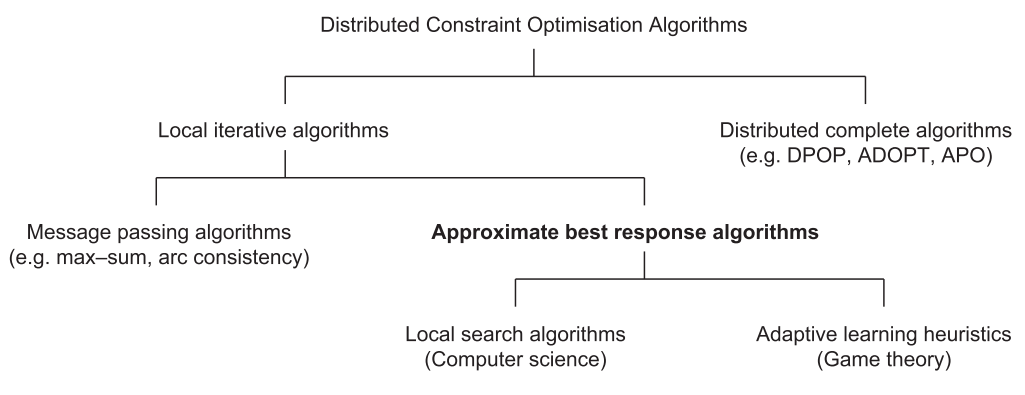
\includegraphics[width=400px]{graphics/overview_algos}
\caption{Categorization of DCO algorithms \cite{Chapman2011}}
\label{fig:categorization}
\end{figure}

\cite{Chapman2011} categorize distributed constraint optimization algorithms into local-iterative and distributed complete algorithms. They further divide local-iterative into message-passing algorithms and approximate best-response algorithms (Figure \ref{fig:categorization}). The following subsections are going to explain the differences between the three categories and introduce the specific algorithms, which have been chosen from these three different approaches for benchmarking. Advantages, as well as disadvantages will be described and which behaviour one can expect of these algorithms under certain parameter configurations.

%Other Approaches: Bee Hive optimization, Genetic Algorithms, .. DynDCOAA, SBDO, Bee Colony algorithm, Ant colony algorithm, adopt, dsa-a, dsa-b stochastic ...\cite{Likhachev}
    
\subsection{Distributed Complete}

%-----------------  Basic Concept and Advantages Disadvantes ----------------------
Distributed complete algorithms always discover a configuration of value assignments for a set of variables that maximizes the global utility function. This completeness guarantee increases the complexity of computation and leads to exponentially growing message numbers or calculations when increasing the amount of variables in a problem. Messages between agents often contain complex structures and constraint problems usually need to be transformed to an extensive graph structure \cite{Chapman2011}. These types of algorithms therefore are not expected to scale well and quickly find qualitative solutions, but they fit well if one wants to find the maximal utility of a problem. 
    %----------------- Chosen algorithm ----------------------
\begin{figure}[H]
\centering
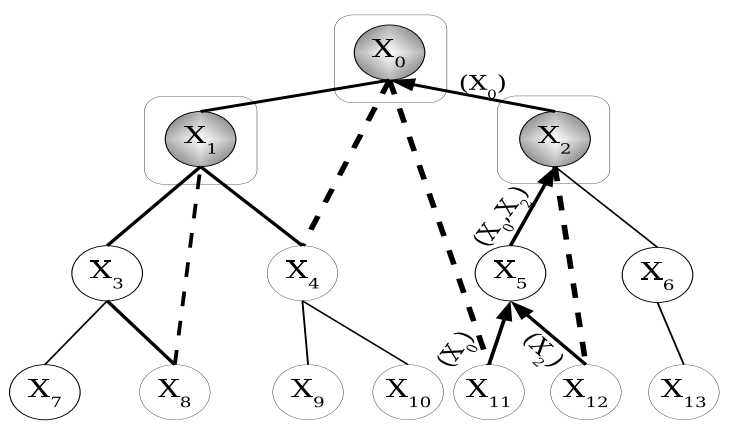
\includegraphics[width=250px]{graphics/pseudotree}
\caption{Pseudotree in DPOP \cite{Petcu2003}}
\label{fig:pseudotree}
\end{figure}

For this thesis, it was decided to implement the Dynamic Programming OPptimization algorithm (DPOP) proposed by \cite{Petcu2003} as a comparison to the local-iterative approaches. In this algorithm, constraint optimization problems need to be converted to a pseudotree (Fig. \ref{fig:pseudotree}), which is a modification of a DFS Tree. The original DCOP graph is transformed in a way that previous neighbours are placed in the same branches of a binary tree. They are connected trough ordinary tree edges and additionally, so-called back-edges between unconnected previous neighbours are established. The leaf nodes propose UTIL messages containing their utility values for each value assignment upwards the tree and the root node sends a VALUE message downwards, containing the best value to choose as a variable state. Nodes in the middle of the tree propagate UTIL and VALUE messages. The message structure is fairly complex as it involves all the utilities of the pseudoparents connected by the back-edges and their context in the graph, which increases the message size exponentially. The number of messages on the other hand is linear \cite{Petcu2003}.

%----------- Dynamics -----------------------
\subsection{Local-Iterative - Best Response}

%-----------------  Basic Concept and Advantages Disadvantes ----------------------
In a local-iterative best-response algorithm, agents only communicate their current state, e.g. their value assignment and react to these value messages in the best possible way from their perspective. The agents are only connected to their neighbours with whom they share constraints and there exists no complex graph structure controlling the message flow \cite{Chapman2011}. Through this local property, the types of algorithms should be inherently scalable as the messages and computations do not increase exponentially. Further, this approach is optimal from a privacy perspective as the neighbours only share their current preference and no other details of their schedule \cite{Chapman2010}. %\cite{Maheswaran} % Achtung muss das richtig paper finden
\newline\newline
%----------------- Chosen algorithm: Structure, Messages --------------------- 
For this thesis, it was decided to implement the Maximum-Gain Messaging algorithm (MGM). In this algorithm, agents  calculate the maximal gain in utility they can achieve when assigning to another value and send this value as a message. If they have the highest gain compared to all received gain messages from their neighbours, the local value is changed. Otherwise the local value stays the same. This algorithm fullfills the anytime property, i.e it can provide a solution at every timepoint during calculation and also reaches good solutions quickly \cite{Chapman2010}. As the decision of an agent depends on a complete set of message of all of its neighbours, this algorithm will supposedly not perform well in asynchronous running mode. This type of algorithm does further not always converge and the deliverance of an optimal solution to a problem is not guaranteed.

\subsection{Local-Iterative - Message Passing}
%-----------------  Basic Concept and Advantages Disadvantes ----------------------
The difference of message-passing to best-response algorithms lays in the fact that the agents send and receive messages containing a specific data structure, which contains the utilities respectively costs that various assignments hold for a local variable. Received messages are used to calculate the next message, which is sent to the connected neighbours. These types of algorithms are - like best-response algorithms - able to provide an acceptable solution in a short period of time, but also share the charasteric to sometimes not converge or not providing an optimal solution \cite{Chapman2011}.
%-----------------  Choosen algorithm ----------------------
\begin{figure}[H]
\centering
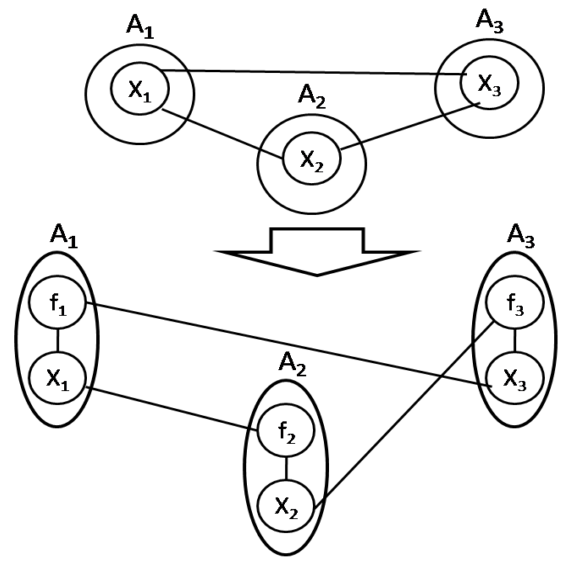
\includegraphics[width=170px]{graphics/factorgraph}
\caption{Conversion of a general DCOP to a factor graph \cite{Zivan2012}}
\label{fig:factorgraph}
\end{figure}

For this thesis, it was decided to implement the MaxSum algorithm introduced by \cite{Farinelli2008}. The algorithm has currently gotten a lot of attention from researchers. For this work, the algorithm is especially interesting because of its proposed abilities in dynamic environments.  \cite{Farinelli2008} wrote in their paper:
\begin{quote}
[...] we note that if messages are continuously propagated,
and the states of the agents are continuously updated, then the algorithm may be applied to dynamic problems where the interactions between agents, or the utilities resulting from these interactions, may change at any time.
\end{quote}

In MaxSum, the original DCOP graph is transformed to a factor graph, which is a form of a bipartite graph and of cyclic nature (Fig. \ref{fig:factorgraph}). After the transformation, an agent is made up of a variable and a function node, whereas variables are connected to all corresponding function nodes of  their previous neighbours. The function nodes are vice versa connected to all previous neighbours of its variable node. 
% ------------- Messages sent --------------------
The messages sent from variable nodes differ from the function nodes. A message from variable to function contains for every value \(d \in D_{x}\) the sum of utilities regarding this value, which the node has received from all connected function nodes. It is important to note that this sum does not include the values provided by the message target. The values are normalized at this point to avoid an infinite increase of the sum of the utilities. A message from a function node to a variable node holds for every value  \(d \in D_{x}\)  the summation of all costs received from all connected variable nodes except the message receiver and the original cost respectively utility of the constraint represented by the function node \cite{Zivan2012}.


    
    
\chapter{Design}
\section{Meeting Scheduling Problem}
\subsection{Formal Definition}
- General problem and definitions
- General constraints Different, Same (sources for that)
- Considerations for all algorithms
\subsection{Problem Generation Considerations}

\section{General Considerations for Dynamics Framework}

\section{Complete - DPOP}
\subsection{Design Considerations}
\subsection{Graph}
\subsection{Vertices}


\section{Local Iterative Best-Respone - Maximum Gain Messaging}
\subsection{Design Considerations}
\subsection{Graph}
\subsection{Vertices}


\section{Local Iterative Message Passing - MaxSum}
\subsection{Design Considerations}
\subsection{Graph}
\subsection{Vertices}

-> Local Iterative
-> Good fit for dynamic
-> Better than the above
-> Fewer information disclosure

\section{Dynamic Environment Module}

%\subsection{Best Response, Local Search - Population-Based Iterated Local Search}
%\subsubsection{Why Population-Based for Dynamic Problems}
%-> Local Iterative
%-> Provides multiple solutions to a problem
%-> Good fit for dynamic -> check which solution is best for changed circumstances
%-> Good fit to stop getting stuck in local optima
%-> Better than the above
%
%
%\subsection{Dynamic, Complete - RSDPOP}
%\subsection{Not local-iterative - SBDO}
%\subsection{Best Response - DSA}
%
%- Distributed, Dynamic, Not-Local-Iterative -> Show what is wrong with this approach regarding dynamic
%
%\subsubsection{Implementation in Signal/Collect}

\section{Testbed, Monitoring}

\chapter{Experiments}
\section{Experiment Design}
The experiments are designed in a two-step procedure accoring to ?

\section{Testing Environment}

\section{Results I: Algorithms Performance Basic}

\subsection{Resilience to dynamic Environments}
- Mainly to proof flaws of the other approaches when it comes to dynamic
\subsection{Solution Quality}
- Static / Dynamic
- Mainly to proof the ability of new approaches to keep stable and reach certain goals
\subsection{Time to Convergence}

\subsection{Scalability}
-  Number of Messages
- Number of Agents
- Mainly to show that local-iterative scales well because the number of messages is low
\subsection{Hardware Requirements}
- Additional layer of argumentation and analysis

\section{Results II: Algorithms Performance after Adjustments}

\subsection{Resilience to dynamic Environments}
\subsection{Time to Convergence}
\subsection{Scalability}
\subsection{Hardware Requirements}
\chapter{Limitations \& Future Work}
\label{c:limitations}

- mehr algorithmen testen
- mehr probleme testen
- generalisieren der aussagen
- benchmarks ausbauen
- distribute to multiple machines was not possible with signal collect at the time
- not fixed participations -> test effect of participations on performance

 
\chapter{Conclusions 3}
\label{c:conclusions} Lorem ipsum dolor sit amet, consectetuer adipiscing
elit. Nullam a tellus. Aliquam commodo dui non ipsum. Duis mollis nisi id
turpis. Donec quis ipsum. Curabitur sed nibh. Morbi suscipit justo quis orci.
Ut massa tortor, ultricies vitae, lacinia eu, facilisis eu, nisl. Nulla mattis
urna sed metus imperdiet ornare. Praesent sodales. Etiam laoreet. Mauris quam
magna, sagittis et, pharetra eget, congue vitae, arcu. Fusce sollicitudin
justo. Suspendisse lectus. Sed lobortis dolor quis lectus scelerisque ornare.
Integer purus. Phasellus vel elit at nibh sagittis lobortis. Aliquam iaculis
malesuada eros. Mauris metus.

In tellus mauris, nonummy eget, vestibulum in, interdum at, nulla. Vestibulum
eu justo. Vivamus lobortis pellentesque arcu. Aliquam enim risus, pulvinar
quis, pulvinar tempor, pharetra vitae, dolor. Aliquam ac sapien. Aenean augue
eros, malesuada nec, tincidunt eget, aliquet bibendum, odio. Maecenas eu est eu
nisi pulvinar bibendum. Lorem ipsum dolor sit amet, consectetuer adipiscing
elit. Pellentesque eleifend varius enim. Ut pharetra diam ac nulla. Aliquam a
turpis ac mi semper porttitor. Vivamus sodales molestie nibh. Vivamus in sapien
sit amet mauris sagittis lobortis. Aenean pretium. Suspendisse eu leo at quam
vehicula aliquam. Nunc a ipsum. Sed placerat fringilla nibh. Aliquam sagittis.
Integer a augue vitae libero elementum pretium. Proin metus.


% *************** Bibliography ***************
\bibliographystyle{apalike}
\bibliography{section-references/thesis_mendeley}

% *************** Appendixes ***************
\appendix
\chapter{Appendix}
\label{a:appendix}

\section{Lorem Ipsum}
Lorem ipsum dolor sit amet, consectetuer adipiscing elit. Nullam a tellus.
Aliquam commodo dui non ipsum. Duis mollis nisi id turpis. Donec quis ipsum.
Curabitur sed nibh. Morbi suscipit justo quis orci. Ut massa tortor, ultricies
vitae, lacinia eu, facilisis eu, nisl. Nulla mattis urna sed metus imperdiet
ornare. Praesent sodales. Etiam laoreet. Mauris quam magna, sagittis et,
pharetra eget, congue vitae, arcu. Fusce sollicitudin justo. Suspendisse
lectus. Sed lobortis dolor quis lectus scelerisque ornare. Integer purus.
Phasellus vel elit at nibh sagittis lobortis. Aliquam iaculis malesuada eros.
Mauris metus.

Lorem ipsum dolor sit amet, consectetuer adipiscing elit. Nullam a tellus.
Aliquam commodo dui non ipsum. Duis mollis nisi id turpis. Donec quis ipsum.
Curabitur sed nibh. Morbi suscipit justo quis orci. Ut massa tortor, ultricies
vitae, lacinia eu, facilisis eu, nisl. Nulla mattis urna sed metus imperdiet
ornare. Praesent sodales. Etiam laoreet. Mauris quam magna, sagittis et,
pharetra eget, congue vitae, arcu. Fusce sollicitudin justo. Suspendisse
lectus. Sed lobortis dolor quis lectus scelerisque ornare. Integer purus.
Phasellus vel elit at nibh sagittis lobortis. Aliquam iaculis malesuada eros.
Mauris metus.

Lorem ipsum dolor sit amet, consectetuer adipiscing elit. Nullam a tellus.
Aliquam commodo dui non ipsum. Duis mollis nisi id turpis. Donec quis ipsum.
Curabitur sed nibh. Morbi suscipit justo quis orci. Ut massa tortor, ultricies
vitae, lacinia eu, facilisis eu, nisl. Nulla mattis urna sed metus imperdiet
ornare. Praesent sodales. Etiam laoreet. Mauris quam magna, sagittis et,
pharetra eget, congue vitae, arcu. Fusce sollicitudin justo. Suspendisse
lectus. Sed lobortis dolor quis lectus scelerisque ornare. Integer purus.
Phasellus vel elit at nibh sagittis lobortis. Aliquam iaculis malesuada eros.
Mauris metus.

Lorem ipsum dolor sit amet, consectetuer adipiscing elit. Nullam a tellus.
Aliquam commodo dui non ipsum. Duis mollis nisi id turpis. Donec quis ipsum.
Curabitur sed nibh. Morbi suscipit justo quis orci. Ut massa tortor, ultricies
vitae, lacinia eu, facilisis eu, nisl. Nulla mattis urna sed metus imperdiet
ornare. Praesent sodales. Etiam laoreet. Mauris quam magna, sagittis et,
pharetra eget, congue vitae, arcu. Fusce sollicitudin justo. Suspendisse
lectus. Sed lobortis dolor quis lectus scelerisque ornare. Integer purus.
Phasellus vel elit at nibh sagittis lobortis. Aliquam iaculis malesuada eros.
Mauris metus.

Lorem ipsum dolor sit amet, consectetuer adipiscing elit. Nullam a tellus.
Aliquam commodo dui non ipsum. Duis mollis nisi id turpis. Donec quis ipsum.
Curabitur sed nibh. Morbi suscipit justo quis orci. Ut massa tortor, ultricies
vitae, lacinia eu, facilisis eu, nisl. Nulla mattis urna sed metus imperdiet
ornare. Praesent sodales. Etiam laoreet. Mauris quam magna, sagittis et,
pharetra eget, congue vitae, arcu. Fusce sollicitudin justo. Suspendisse
lectus. Sed lobortis dolor quis lectus scelerisque ornare. Integer purus.
Phasellus vel elit at nibh sagittis lobortis. Aliquam iaculis malesuada eros.
Mauris metus.


% *************** Back matter ***************
\backmatter

\normalfont
\clearpage
\listoffigures

\clearpage
\listoftables


\end{document}